\documentclass[11pt,handout,xcolor=pdftex,dvipsnames,table]{beamer}
\usefonttheme[onlymath]{serif}
\usetheme{default}
%\usetheme{Darmstadt}
%\usepackage{times}
%\usefonttheme{structurebold}

\usepackage[english]{babel}
%\usepackage[table]{xcolor}
\usepackage{amsmath}
\usepackage{pgf,pgfarrows,pgfnodes,pgfautomata,pgfheaps}
\usepackage{amsmath,amssymb,setspace}
\usepackage[latin1]{inputenc}
\usepackage[T1]{fontenc}
\usepackage{relsize}

\usepackage{pxfonts}

\usepackage[absolute,overlay]{textpos} 
\newenvironment{reference}[2]{% 
  \begin{textblock*}{\textwidth}(#1,#2) 
      \footnotesize\it\bgroup\color{red!50!black}}{\egroup\end{textblock*}} 

\DeclareMathSizes{10}{10}{6}{6} 


\title [Bootstrap]{Delta Method, Bootstrap, and Cross Validation}
\author{C.Conlon}
\institute{Microeconometrics}
\date{\today}
\setbeamerfont{equation}{size=\tiny}
\begin{document}

\begin{frame}
\titlepage
\end{frame}

\begin{frame}{Bootstrap and Delta Method}
\begin{itemize}
\item We know how to construct confidence intervals for parameter estimates:  $\hat{\theta}_k \pm 1.96 SE(\hat{\theta}_k)$
\item Often we are asked to construct standard errors or confidence intervals around model outputs that are not just parameter estimates: ie:  $g(x_i,\hat{\theta})$.
\item Sometimes we can't even write $g(x_i,\theta)$ as an explicit function of $\theta$ ie: $\Psi(g(x_i,\theta),\theta) = 0$.
\item Two options:
\begin{enumerate}
\item Delta Method
\item Bootstrap
\end{enumerate}
\end{itemize}
\end{frame}

\begin{frame}{Delta Method}
Delta method works by considering a \alert{Taylor Expansion} of $g(x_i,\theta)$.
\begin{eqnarray*}
g(z) \approx g(z_0) + g'(z_0)(z-z_0) + o(||z-z_0||)
\end{eqnarray*}
Assume that $\theta_n$ is asymptotically normally distributed so that:
\begin{eqnarray*}
\sqrt{n} (\theta_n - \theta_0) \sim N(0,\Sigma)
\end{eqnarray*}
(How do we get this: OLS? GMM? MLE?).\\

Then we have that 
\begin{eqnarray*}
\sqrt{n} (g(\theta_n) - g(\theta_0)) \sim N(0,D(\theta)' \Sigma  D(\theta))
\end{eqnarray*}
Where $D(\theta) = \frac{\partial g(x_i, \theta)}{\partial \theta}$ is the Jacobian of $g$ with respect to theta evaluated at $\theta$.\\
We need $g$ to be continuously differentiable around the center of our expansion $\theta$.
\end{frame}


\begin{frame}{Delta Method: Examples}
Start with something simple: $Y= \overline{X}_1\cdot \overline{X}_2$ with $(X_{1i},X_{2i}) \sim IID$.
We know the CLT applies so that:
\begin{eqnarray*}
\sqrt{n}
\begin{pmatrix}
\overline{X}_1 - \mu_1\\
\overline{X}_2 - \mu_2
\end{pmatrix} &\sim  N
\begin{bmatrix}
\begin{pmatrix}
0\\
0
\end{pmatrix},
\Sigma
\end{bmatrix}
\end{eqnarray*}
The Jacobian is just $D(\theta) =  \begin{pmatrix}\frac{\partial g(\theta)}{\partial \theta_1} \\ \frac{\partial g(\theta)}{\partial \theta_2}  \end{pmatrix} =  \begin{pmatrix}s_2\\ s_1 \end{pmatrix}$\\
So,
\begin{eqnarray*}
V(Y) = D(\theta)' \Sigma D(\theta) =\begin{pmatrix} \mu_2 & \mu_1 \end{pmatrix}  \begin{pmatrix} \sigma_{11} & \sigma_{12} \\ \sigma_{21} & \sigma_{22} \end{pmatrix} \begin{pmatrix} \mu_2 \\\mu_1  
\end{pmatrix} \\
\sqrt{n} ( \overline{X}_1 \overline{X}_2 - \mu_1 \mu_2) \sim N(0,\mu_2^2 \sigma_{11}^2 + 2 \mu_1 \mu_2 \sigma_{12}  + \mu_1^2 \sigma_{22}^2)
\end{eqnarray*}
\end{frame}

\begin{frame}{Delta Method: Examples}
Think about a simple logit:
\begin{eqnarray*}
P(Y_i=1 | X_i ) = \frac{\exp^{\beta_0 + \beta_1 X_i}}{1+\exp^{\beta_0 + \beta_1 X_i}}  \quad P(Y_i=0 | X_i ) = \frac{1}{1+\exp^{\beta_0 + \beta_1 X_i}} 
\end{eqnarray*}
Remember the ``trick'' to use GLM (log-odds):
\begin{eqnarray*}
\log P(Y_i=1 | X_i) - \log P(Y_i=0 | X_i) = \beta_0 + \beta_1 X_i
\end{eqnarray*}
\begin{itemize}
\item Suppose that we have estimated $\hat{\beta_0},\hat{\beta_1}$ via GLM/MLE but we want to know the confidence interval for the probability: $P(Y_i=1 | X_i,\hat{\theta})$
\item The derivatives are a little bit tricky, but the idea is the same.
\item This is what STATA should be doing when you type: \tt{mfx, compute}
\end{itemize}
\end{frame}

\begin{frame}{Delta Method: Other Examples}
Often we have a regression like:
\begin{eqnarray*}
log Y_i = \beta_0 + \beta_1 X_i + \gamma Income_i + \epsilon_i
\end{eqnarray*}
And we are interested in $\beta_1 / \gamma$ so that we have $\beta_i$ in units of ``dollars''. Again Delta Method Works fine here.\\
\end{frame}


\begin{frame}{Delta Method: Some Failures}
But we need to be careful.  Suppose that $\theta \approx 0$ and 
\begin{itemize}
\item $g(x)  = |X|$
\item $g(x)  = 1/X$
\item $g(x)  = \sqrt{X}$
\end{itemize}
These situations can arise in practice when we have weak instruments or other problems.
\end{frame}

\begin{frame}{Bootstrap}
\begin{itemize}
\item Bootstrap takes a different approach.
\begin{itemize}
\item Instead of estimating $\hat{\theta}$ and then using a first-order Taylor Approximation...
\item What if we directly tried to construct the \alert{sampling distribution} of $\hat{\theta}$?
\end{itemize}
\item Our data $(X_1,\ldots,X_n) \sim P$ are drawn from some measure $P$
\begin{itemize}
\item We can form a \alert{nonparametric estimate} $\hat{P}$ by just assuming that each $X_i$ has weight $\frac{1}{n}$.
\item We can then simulate a new sample $X^{*} = (X_1^{*},\ldots X_n^{*}) \sim \hat{P}$.
\begin{itemize}
\item Easy: we take our data and construct $n$ observations by \alert{sampling with replacement} 
\end{itemize}
\item Compute whatever statistic of $X^{*}$, $S(X^*)$ we would like.
\begin{itemize}
\item Could be the OLS coefficients $\beta_1^{*},\ldots, \beta_k^{*}$.
\item Or some function $\beta_1^{*}/\beta_2^{*}$.
\item Or something really complicated: estimate parameters of a game $\hat{\theta}^*$ and now find Nash Equilibrium of the game $S(X^{*},\hat{\theta^*})$ changes.
\end{itemize}
\item Do this $B$ times and calculate at $Var(S_b)$ or $CI(S_1,\ldots, S_b)$.
\end{itemize}
\end{itemize}
\end{frame}


\begin{frame}{Bootstrap: Bias Correction}
\small
The main idea is that $\hat{\theta}^{1*},\ldots, \hat{\theta}^{B*}$ approximates the \alert{sampling distribution} of $\hat{\theta}$. There are lots of things we can do now:
\begin{itemize}
\item We already saw how to calculate $Var(\hat{\theta}^{1*},\ldots, \hat{\theta}^{B*})$.
\begin{eqnarray*}
\frac{1}{B-1} \sum_{b=1}^B (\hat{\theta}_{(b)}^* - \overline{\theta^{*}})^2
\end{eqnarray*}

\item Calculate $E(\hat{\theta}^{*}_{(1)},\ldots, \hat{\theta}^{*}_{(B)}) = \overline{\theta^{*}} = \frac{1}{B} \sum_{b=1}^B \hat{\theta}_{(b)}^*$.
\begin{itemize}
\item We can use the estimated bias to \alert{bias correct} our estimates
\begin{eqnarray*}
Bias(\hat{\theta}) &=&E[\hat{\theta}] - \theta \\
Bias_{bs}(\hat{\theta}) &=&\overline{\theta^{*}} -\hat{\theta}
\end{eqnarray*}
Recall $\theta = E[\hat{\theta}] - Bias[\hat{\theta}]$:
\begin{eqnarray*}
\hat{\theta}- Bias_{bs}(\hat{\theta}) = \hat{\theta}-(\overline{\theta^{*}}-\hat{\theta}) = 2 \hat{\theta} - \overline{\theta^{*}}
\end{eqnarray*}
\end{itemize}
\item Correcting bias isn't for free - variance tradeoff!
\item Linear models are (hopefully) unbiased, but most nonlinear models are \alert{consistent but biased}.
\end{itemize}

\end{frame}

\begin{frame}{Bootstrap: Confidence Intervals}
There are actually three ways to construct bootstrap CI's:
\begin{enumerate}
\item Obvious way: sort  $\hat{\theta}^{*}$ then take $CI: [\hat{\theta}^{*}_{\alpha/2},\hat{\theta}^{*}_{1-\alpha/2}]$.
\item Asymptotic Normal:  $CI: \hat{\theta} \pm 1.96 \sqrt{V(\hat{\theta}^{*})}$. (CLT).
\item Better Way: let $W= \hat{\theta} -\theta$. If we knew the distribution of $W$ then: $Pr(w_{1-\alpha/2} \leq W \leq w_{\alpha/2})$:
\begin{eqnarray*}
CI: [\hat{\theta} -w_{1-\alpha/2}, \hat{\theta} -w_{\alpha/2}]
\end{eqnarray*}
We can estimate with $W^{*} = \hat{\theta}^{*} - \hat{\theta}$.
\begin{eqnarray*}
CI: [\hat{\theta} -w^*_{1-\alpha/2}, \hat{\theta} -w^*_{\alpha/2}] = [2 \hat{\theta} -\theta^*_{1-\alpha/2}, 2 \hat{\theta} -\theta^*_{\alpha/2}]
\end{eqnarray*}
Why is this preferred? Bias Correction!
\end{enumerate}

\end{frame}


\begin{frame}{Bootstrap: Why do people like it?}
\begin{itemize}
\item Econometricians like the bootstrap because under certain conditions it is \alert{higher order efficient} for the confidence interval construction (but not the standard errors).
\begin{itemize}
\item Intuition: because it is non-parametric it is able to deal with more than just the first term in the Taylor Expansion (actually an \alert{Edgeworth Expansion}).
\item Higher-order asymptotic theory is best left for real econometricians!
\end{itemize}
\item Practitioner's like the bootstrap because it is easy.
\begin{itemize}
\item If you can estimate your model once in a reasonable amount of time, then you can construct confidence intervals for most parameters and model predictions.
\end{itemize}
\end{itemize}
\end{frame}

\begin{frame}{Bootstrap: When Does It Fail?}
\begin{itemize}
\item Bootstrap isn't magic. If you are constructing standard errors for something that isn't asymptotically normal, don't expect it to work!
\item The Bootstrap exploits the notion that your sample is IID (by sampling with replacement). If IID does not hold, the bootstrap may fail (but we can sometimes fix it!).
\item Bootstrap depends on asymptotic theory. In small samples weird things can happen. We need $\hat{P}$ to be a good approximation to the true $P$ (nothing missing).
\end{itemize}
\end{frame}

\begin{frame}{Bootstrap: Variants}
The bootstrap I have presented is sometimes known as the \alert{nonparametric bootstrap} and is the most common one.
\begin{description}
\item[Parametric Bootstrap] ex: if $Y_i = \beta_0 + \beta_1 X_i + \epsilon_i$ then we can estimate $(\hat{\beta}_0,\hat{\beta}_1)$ via OLS.\\
 Now we can generate a bootstrap sample by drawing an $x_i$ at random with replacement $\hat{\beta}_0 + \hat{\beta}_1$ and then drawing \alert{independently} from the distribution of estimated residuals $\hat{\epsilon}_i$.
 \item[Wild Bootstrap] Similar to parametric bootstrap but we rescale $\epsilon_i$ to allow for \alert{heteroskedasticity}
\item[Block Bootstrap] For correlated data (e.g.: time series). Blocks can be overlapping or not.  
\end{description}
\end{frame}

\begin{frame}{Bootstrap vs Delta Method}
\begin{itemize}
\item Delta Method works best when working out Jacobian $D(\theta)$ is easy and statistic is well approximated with a linear function (not too curvy).
\item I would almost always advise Bootstrap unless:
\begin{itemize}
\item Delta method is trivial e.g.: $\beta_1 / \beta_2$ in linear regression.
\item Computing model takes many days so that 10,000 repetitions would be impossible.
\end{itemize}
\item Worst case scenario: rent time on Amazon EC2!
\begin{itemize}
\item I ``bought'' over \$1,000 of standard errors recently.
\end{itemize}
\item But neither is magic and both can fail!
\end{itemize}
\end{frame}

\begin{frame}{Cross Validation}
Cross Validation appears superficially similar to bootstrap but asks a different question.
\begin{itemize}
\item Bootstrap tries to construct an empirical analogue to the sampling distribution of $\hat{\theta}$.
\item CV tries to measure what the expected out of sample (OOS or EPE) prediction error of a new never seen before dataset.
\item The main consideration is to prevent \alert{overfitting}.
\begin{itemize}
\item In sample fit is always going to be maximized by the most complicated model.
\item OOS fit might be a different story.
\item 1-NN might do really well in-sample, but with a new sample might perform badly.
\end{itemize}
\end{itemize}
\end{frame}

\begin{frame}{Sample Splitting/Holdout Method and CV}
Cross Validation is actually a more complicated version of \alert{sample splitting} that is one of the organizing principles in machine learning literature.

\begin{description}
\item[Training Set] This is where you estimate parameter values.
\item[Validation Set] This is where you choose a model- a bandwidth $h$ or tuning parameter $\lambda$ by computing the error.
\item[Test Set] You are only allowed to look at this after you have chosen a model. \alert{Only Test Once}: compute the error again on fresh data.
\end{description}
\begin{itemize}
\item Conventional approach is to allocate 50-80\% to training and 10-20\% to Validation and Test.
\item Sometimes we don't have enough data to do this reliably.
\end{itemize}
\end{frame}

\begin{frame}{Sample Splitting/Holdout Method}
\begin{center}
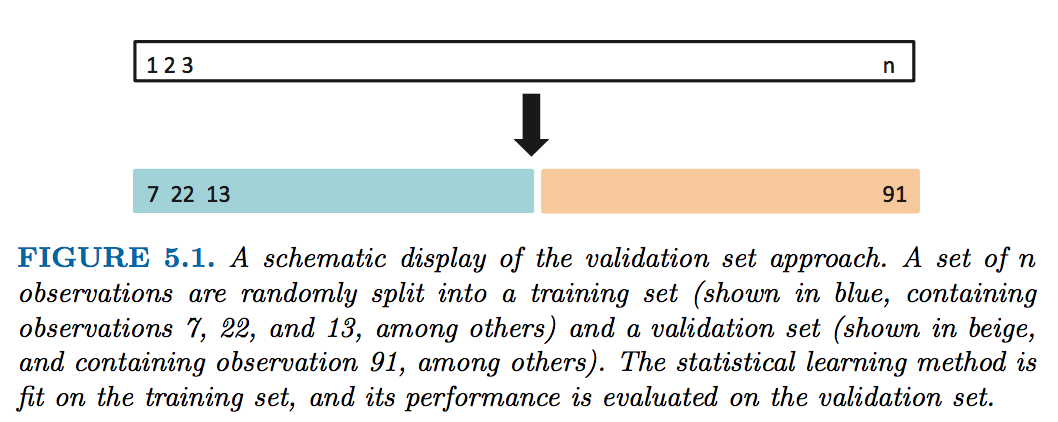
\includegraphics[width=4.5in]{./resources/split-sample}
\end{center}
\end{frame}

\begin{frame}{Challenge with Sample Splitting}
\begin{center}
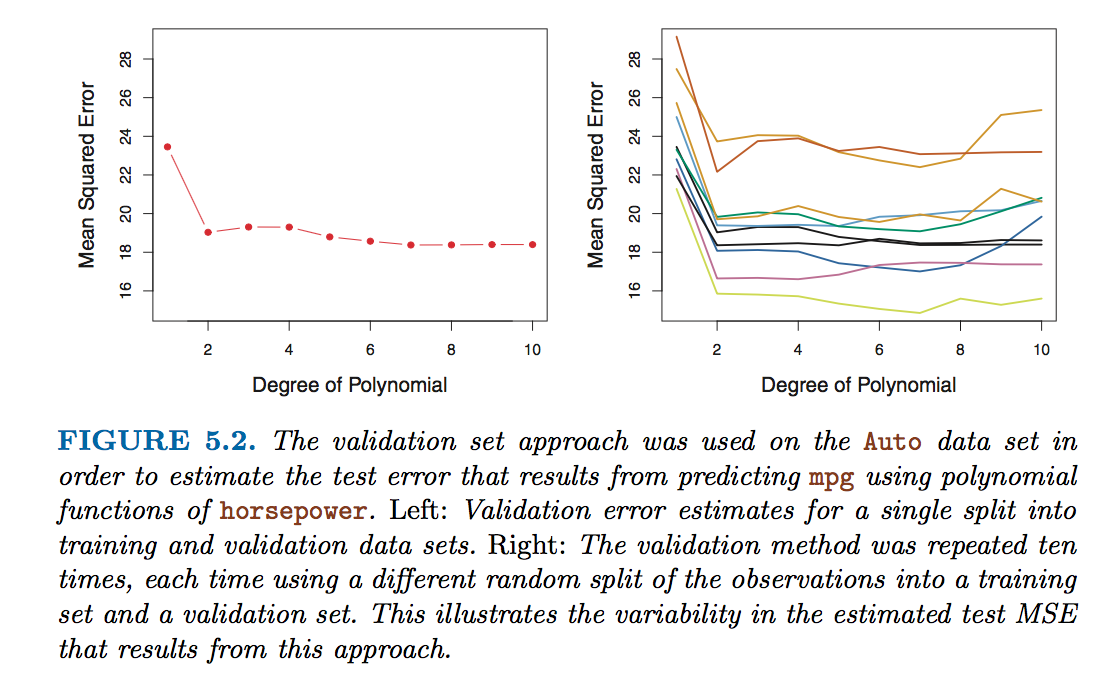
\includegraphics[width=4.5in]{./resources/validation-10fold}
\end{center}
\end{frame}


\begin{frame}{Cross Validation}
\begin{center}
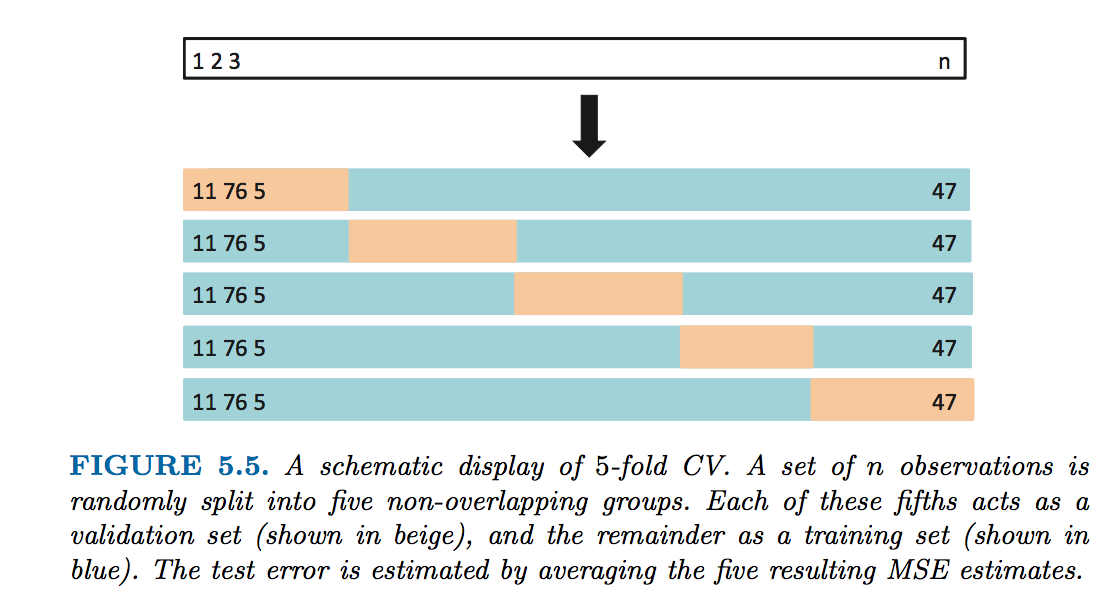
\includegraphics[width=4.5in]{./resources/split-cv5}
\end{center}
\end{frame}

\begin{frame}{$k$-fold Cross Validation}
\begin{itemize}
\item Break the dataset into $k$ equally sized ``folds'' (at random).
\item Withhold $i=1$ fold
\begin{itemize}
\item Estimate the model parameters $\hat{\theta}^{(-i)}$ on the remaining $k-1$ folds
\item Predict $\hat{y}^{(-i)}$ using $\hat{\theta}^{(-i)}$ estimates for the $i$th fold (withheld data).
\item Compute $MSE_i =\frac{1}{k \cdot N} \sum_j (y^{(-i)}_j -\hat{y}^{(-i)}_j)^2$.
\item Repeat for $i=1,\ldots,k$.
\end{itemize}
\item Construct $\widehat{MSE}_{k,CV} = \frac{1}{k} \sum_i MSE_{i}$
\end{itemize}
\end{frame}

\begin{frame}{Leave One Out Cross Validation (LOOCV)}
Same as $k$-fold but with $k=N$.
\begin{itemize}
\item Withhold a single observation $i$
\item Estimate $\hat{\theta}_{(-i)}$.
\item Predict $\hat{y}_i$ using $\hat{\theta}^{(-i)}$ estimates
\item Compute $MSE_i =\frac{1}{N} \sum_j (y_i -\hat{y}_i(\hat{\theta}^{(-i)}))^2$.
\end{itemize}
\vspace{0.2cm}
Note: this requires estimating the model $N$ times which can be costly.
\end{frame}



\begin{frame}{Cross Validation}
\begin{center}
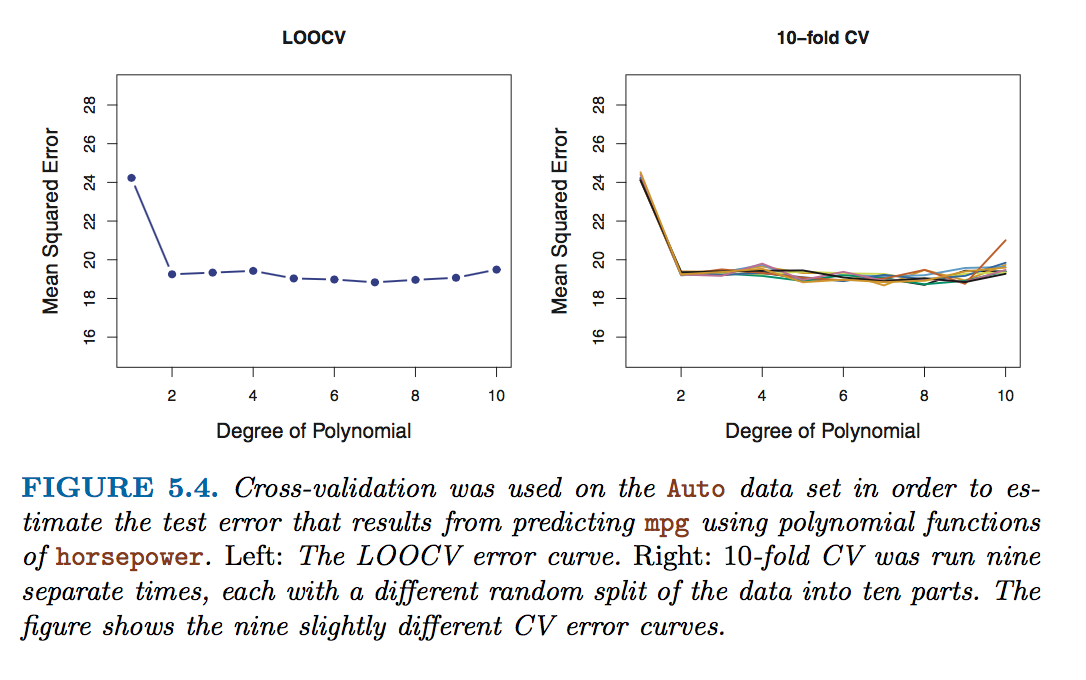
\includegraphics[width=4.5in]{./resources/comparison-cv}
\end{center}
\end{frame}

\begin{frame}{Cross Validation}
\begin{itemize}
\item Main advantage of cross validation is that we use all of the data in both \alert{estimation} and in \alert{validation}.
\begin{itemize}
\item For our purposes validation is mostly about choosing the right bandwidth or tuning parameter.
\end{itemize}
\item We have much lower variance in our estimate of the OOS mean squared error.
\begin{itemize}
\item Hopefully our bandwidth choice doesn't depend on randomness of splitting sample.
\end{itemize}
\end{itemize}
\end{frame}



\begin{frame}{Test Data}
\begin{itemize}
\item In Statistics/Machine learning there is a tradition to withhold 10\% of the data as \alert{Test Data}.
\item This is \alert{completely new data} that was not used in the CV procedure.
\item The idea is to report the results using this test data because it most accurately simulates true OOS performance.
\item We don't do much of this in economics.\\
 (Should we do more?)
\end{itemize}
\end{frame}





\end{document}